\documentclass{article}

\usepackage{amsmath, amsfonts, amsthm, amssymb} 
\newcommand{\dd}{\mathrm{d}}
\newcommand{\RR}{\mathbb{R}}
\usepackage{listings}
\usepackage{graphicx}
\usepackage{float}
\usepackage{subfigure}
\usepackage{geometry}
\usepackage{hyperref}

\geometry{
	paper=a4paper, 
	top=2.5cm,
	bottom=2.5cm, 
	left=2.5cm, 
	right=3cm,
	headsep=0.75cm, 
}
\title{ROB 501 HW1}
\author{Yulun Zhuang \\ \href{mailto:yulunz@umich.edu}{yulunz@umich.edu}}
\date{\today}

\begin{document}

\maketitle

\section{}

Let $A$ be an $n \times m$ matrix and $B$ an $m \times p$ matrix. Denote the $i$-th row of $A$ by $a_i$ and the $j$-th column of $B$ by $b_j$.

\begin{align}
    AB = &
    \begin{bmatrix}
        a_1\\a_2\\\vdots\\a_n
    \end{bmatrix}
    \begin{bmatrix}
        b_1 & b_2 & \dots &b_p
    \end{bmatrix}\\
    = &
    \begin{bmatrix}
        a_1b_1 & a_1b_2 & \dots & a_1b_p\\
        a_2b_1 & a_2b_2 & \dots & a_2b_p \\
        \vdots & \vdots & \ddots& \vdots\\
        a_nb_1 & a_nb_2 & \dots & a_nb_p\\
    \end{bmatrix}\label{eq:2}
\end{align}

\subsection{}
According to eq \eqref{eq:2}, we can collect $b_j$ for each column of $AB$, which leads to

\begin{align*}
    AB = &
    \begin{bmatrix}
        a_1\\a_2\\\vdots\\a_n
    \end{bmatrix}
    b_1
    +
    \begin{bmatrix}
        a_1\\a_2\\\vdots\\a_n
    \end{bmatrix}
    b_2
    +
    \dots
    +
    \begin{bmatrix}
        a_1\\a_2\\\vdots\\a_n
    \end{bmatrix}
    b_p\\
    = &
    \begin{bmatrix}
        Ab_1 & Ab_2 & \dots & Ab_p
    \end{bmatrix}
\end{align*}

\subsection{}
According to eq \eqref{eq:2}, we can collect $a_i$ for each row of $AB$, which leads to

\begin{align*}
    AB = & 
    a_1
    \begin{bmatrix}
        b_1 & b_2 & \dots &b_p
    \end{bmatrix}
    +\\ &
    a_2
    \begin{bmatrix}
        b_1 & b_2 & \dots &b_p
    \end{bmatrix}
    +
    \dots
    +\\ &
    a_n
    \begin{bmatrix}
        b_1 & b_2 & \dots &b_p
    \end{bmatrix}\\
    = & 
    \begin{bmatrix}
        a_1B \\ a_2B \\ \vdots \\ a_nB
    \end{bmatrix}
\end{align*}

\subsection{}
According to eq \eqref{eq:2}, the entry of $i$-the row and $j$-th column of $AB$ is $a_ib_j$, i.e. 

$$
[AB]_{ij} = a_ib_j
$$

\section{}

Given $A\in \RR^{n\times n}$, $tr(A) = \sum_{i=1}^{n}a_ii$.

\subsection{}

\begin{align*}
    A = & 
    \begin{bmatrix}
        1 & 2 & 3\\
        4 & 5 & 6\\
        7 & 8 & 9
    \end{bmatrix}\\
    tr(A) = & 1+5+9 = 15
\end{align*}

\subsection{}

\begin{align*}
    x = &
    \begin{bmatrix}
        x_1 \\ x_2 \\ \vdots \\ x_n
    \end{bmatrix}
    \in \RR ^n\\
    xx^T = &
    \begin{bmatrix}
        x_1 \\ x_2 \\ \vdots \\ x_n
    \end{bmatrix}
    \begin{bmatrix}
        x_1 & x_2 & \dots & x_n
    \end{bmatrix}\\
    = &
    \begin{bmatrix}
        x_1x_1 & x_1x_2 & \dots & x_1x_n\\
        x_2x_1 & x_2x_2 & \dots & x_2x_n \\
        \vdots & \vdots & \ddots& \vdots\\
        x_nx_1 & x_nx_2 & \dots & x_nx_n\\
    \end{bmatrix}\\
    tr(xx^T) = &
    \sum_{i=1}^n x_i x_i
\end{align*}

\subsection{}

Given $K\in \RR^{n\times m}$ and $Q\in \RR^{n \times n}$. Let $k_i$ be the i-th column of $K$.

\begin{align*}
    K^TQK = &
    \begin{bmatrix}
        k_1^T\\k_2^T\\\vdots\\k_m^T
    \end{bmatrix}
    Q
    \begin{bmatrix}
        k_1 & k_2 & \dots & k_m
    \end{bmatrix}\\
    = &
    \begin{bmatrix}
        k_1^TQ\\k_2^TQ\\\vdots\\k_m^TQ
    \end{bmatrix}
    \begin{bmatrix}
        k_1 & k_2 & \dots & k_m
    \end{bmatrix}\\
    = &
    \begin{bmatrix}
        k_1^TQk_1 & k_1^TQk_2 & \dots & k_1^TQk_m\\
        k_2^TQk_1 & k_2^TQk_2 & \dots & k_2^TQk_m \\
        \vdots & \vdots & \ddots& \vdots\\
        k_m^TQk_1 & k_m^TQk_2 & \dots & k_m^TQk_m\\
    \end{bmatrix}\\
    tr(K^TQK) = &\sum_{i=1}^m k_i^TQk_i
\end{align*}

\section{}

A real matrix $M$ is symmetric if it is equal to its transpose: $M^T = M$.
\subsection{}
\begin{align*}
    M = 
    \begin{bmatrix}
        2 & 1 \\ 1 & 3
    \end{bmatrix}& \\
    det(M - \lambda I) = & 0\\
    \left| 
        \begin{matrix}
            2-\lambda & 1 \\ 1 & 3-\lambda 
        \end{matrix}
    \right|
    = & 0\\
    \Rightarrow \lambda_1 = \frac{5 - \sqrt{5}}{2},\ \lambda_2 =&  \frac{5 + \sqrt{5}}{2}
\end{align*}

\subsection{}

When $\lambda=\lambda_1$,

\begin{align*}
    (M - \lambda_1 I) v_1= & 0\\
    \Rightarrow v_1 = &
    \begin{bmatrix}
        1 \\ \frac{1-\sqrt{5}}{2}
    \end{bmatrix}
\end{align*}
When $\lambda=\lambda_2$,

\begin{align*}
    (M - \lambda_2 I) v_2= & 0\\
    \Rightarrow v_2 = &
    \begin{bmatrix}
        1 \\ \frac{1 + \sqrt{5}}{2}
    \end{bmatrix}
\end{align*}

$$
v_1^Tv_2 = 0
$$

\subsection{}

Show that $M = A^T A$ is symmetric for any real $n \times m$ matrix A.

\begin{align*}
    M^T = (A^TA)^T = A^TA = M
\end{align*}
\\
Thus, $\forall A\in \RR^{n\times m},\ M = A^TA$ is symmetric.

\subsection{}
\begin{itemize}
    \item The inner product of eigenvectors $v_i^Tv_i$  with $i\neq j$ is \textbf{zero}.
    \item The sum of all eigenvalues is the \textbf{same} as the trace of the matrix.
    \item The product of all eigenvalues is the \textbf{same} as the determinant of the matrix.
\end{itemize}

\section{}

Given $X\sim N(\mu, \sigma^2)$, 
\begin{align}
    f_X(x) = \frac{1}{\sigma\sqrt{2\pi}}exp(-\frac{(x-\mu)^2}{2\sigma^2})
\end{align}

\subsection{}

\begin{figure}[H]
    \centering
        \textsf{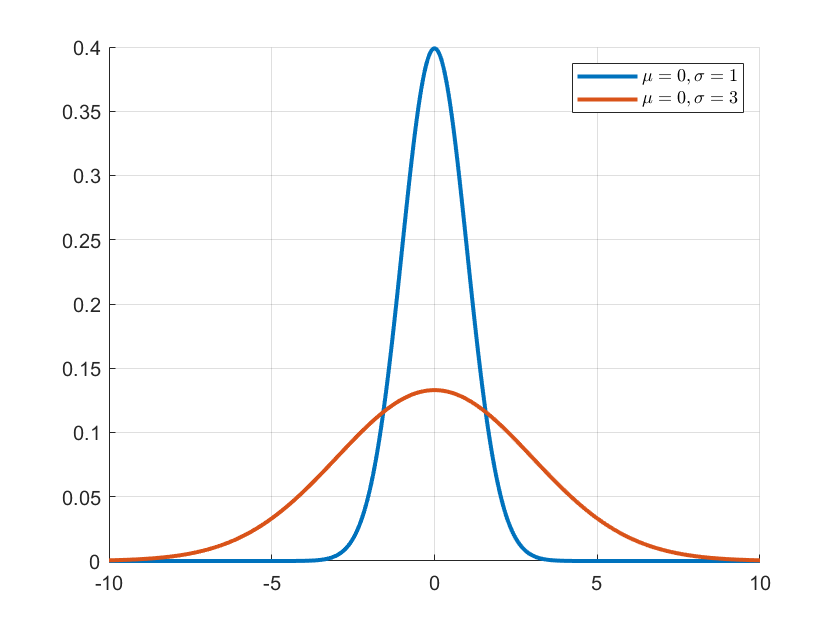
\includegraphics[width=0.6\columnwidth]{hw1-fig1.png}}
        \caption{Density plots for different $\sigma$}
        \label{fig: 1}
\end{figure}

\subsection{}
For $\mu = 4$ and $\sigma = 5$,

\begin{align*}
    P\left\{X\ge 4 \right\} =& \int^\infty_4 f_X(x) = 0.3446\\
    P\left\{-2\le X \le 4 \right\} = & \int^4_{-2} f_X(x) = 0.4436\\
    P\left\{X\in A|A = [-2, 4] \cup [8, 100]\right\} =& \int^4_{-2} f_X + \int^{100}_{8} f_X = 0.5586
\end{align*}

\subsection{}
Given $Y = 2X+4$, we have $\mu^\prime = 2\mu +4 = 8$ and $\sigma^\prime = 2\sigma = 10$. Thus

$$
f_X(x) = \frac{1}{10\sqrt{2\pi}}exp(-\frac{(x-8)^2}{200})
$$


\section{}

Given $f_{XY}(x, y) = K(x+y)^2,\ 0\le x\le 1,\ 0\le y\le 2$.

\subsection{}
\begin{align*}
    \int_0^1 \int_0^2 K(x+y)^2 d y d x = & 1\\
    \int_0^1 K\left(2 x^2+4 x+\frac{8}{3}\right) d x = & 1\\
    K\left(\frac{2}{3}+2+\frac{8}{3}\right)= & 1\\
    K = & \frac{3}{16}
\end{align*}

\subsection{}
Marginal densities and distributions

\begin{align*}
    f_Y(y) &=\int_0^1 \frac{3}{16}(x+y)^2 d x \\
    &=\frac{3}{16} y^2+\frac{3}{16} y+\frac{1}{16} \\
    F_Y(y) &= \int^y_{0}f_Y(v)dv\\
    &= \frac{1}{16}y^3+\frac{3}{32}y^2+\frac{1}{16}y\\
    f_X(x) &=\int_0^2 \frac{3}{16}(x+y)^2 d y \\
    &=\frac{3}{8} x^2+\frac{3}{4} x+\frac{1}{2}\\
    F_X(x) &= \int^x_{0}f_X(u)du\\
    &= \frac{1}{8}x^3+\frac{3}{8}x^2+\frac{1}{4}x\\
\end{align*}
\subsection{}
Conditional densities and distributions

\begin{align*}
    f_{X|Y}(x|Y=y) =& \frac{f_{XY}(x, y)}{f_Y(y)} = \frac{(x+y)^2}{y^2+y+1/3}\\
    F_{X|Y}(x|Y=y) =& \int_0^x f_{X|Y}(u|Y=y)du = \frac{ x^3 + 3yx^2 + 3y^2x}{3y^2 + 3y + 1}
\end{align*}


\section{}

\begin{align*}
    min\ & x_1^2+x_2^2\\
    s.t.\ & x_1 + 3x_2 = 4
\end{align*}

where $x_1, x_2 \in \RR$.
\\
Let $$f(x)=x_1^2+x_2^2,\ g(x)=x_1+3 x_2-4$$ 

and $$L(x, \lambda) =  f(x)-\lambda g(x)$$ 

where $\lambda>0$.
\begin{align*}
    \nabla L&=\nabla f(x)-\lambda \nabla g(x)\\
    &=\left[\begin{array}{l}
    2 x_1 \\
    2 x_2
    \end{array}\right]-\lambda\left[\begin{array}{l}
    1 \\
    3
    \end{array}\right]\\
    &=\left[\begin{array}{l}
    2 x_1-\lambda \\
    2 x_2-3 \lambda
    \end{array}\right]
\end{align*}
\\
Solve $\nabla L = \mathbf 0$,
$$
\left\{\begin{array} { l } 
    { 2 x _ { 1 } - \lambda = 0 } \\
    { 2 x _ { 2 } - 3 \lambda = 0 } \\
    { x _ { 1 } + 3 x _ { 2 } = 4 }
    \end{array} \Rightarrow \left\{\begin{array}{l}
    x_1=2/5 \\
    x_2=6/5 \\
    \lambda=4/5
\end{array}\right.\right.
$$
\\
Check the Hessian matrix
$$
\nabla^2L = 
\begin{bmatrix}
    2 & 0\\ 0 & 2
\end{bmatrix}
$$

which is positive definite. Thus $x_0 = [2/5,\ 6/5]^T$ is a local minimum point of $f(x)$.


\section{}

\subsection{}
Marginal densities and distributions
\begin{align*}
    X \sim & N(1, 3)\\    
    f_X(x) =& \frac{1}{\sqrt{6\pi}}exp(-\frac{(x-1)^2}{6})\\ 
    F_X(x) =& \int^x_{-\infty} \frac{1}{\sqrt{6\pi}}exp(-\frac{(u-1)^2}{6})du\\
    Y \sim &N(2, 2)\\    
    f_Y(y) =& \frac{1}{2\sqrt{\pi}}exp(-\frac{(y-2)^2}{4})\\    
    F_Y(y) =& \int^y_{-\infty} \frac{1}{2\sqrt{\pi}}exp(-\frac{(v-2)^2}{4})dv
\end{align*}

\end{document}